\cleardoublepage
\chapter{Implementation??} \label{chap:trans}
\todo[inline,color=red!40]{*1-Introduction}
\todo[inline,color=yellow!40]{*2-Measuring Sensors}
\todo[inline,color=yellow!40]{*3-Real Signal Analysis}

\section{Introduction}
\section{Sensors} %Change latter 
As the system is stimulated by hitting with a hammer on his side surface, the LPG bottle will produce internal vibration and also a sound, for the different levels, and according to what was stated in the section \ref{sec:LPGModel}, will produce a different response in his frequency analysis. Since the response can be measured by the system vibration or the sound that is produced, when hitting the side surface, that allows different approaches to measure the system response.\\
The first and obvious approach is to use a microphone, to capture the sound produced, proceeding with his analysis in frequency. This his one of the easiest approaches, and is going to be used in a first stage to verify the response of the system, in this case it won't be necessary to developed additional hardware, a external microphone is going to be used with this purpose, more about the setup in \ref{sec:MIC}.\\

\section{Real Signal analysis}\label{sec:MIC}
As mentioned in \ref{subsec:SOAExpRes}, for different LPG bottles, the response to a external impulse will cause different vibration and thus, a different curve in the relation between weight and frequency. So the first step, is to evaluate this relation in the set of LPG bottles available[reference to the image of the bottles], in this case was available 3 LPG bottles, one empty, another half filled and the last completely filled, according to the 80\% rule, with water inside for safety reasons. The easiest way to perform this test is using a microphone, a hammer(or another object to hit the LPG bottle) and MatLab***. To capture the sound produced by hitting the bottle, the microphone of a Phone was used in addition with MatLab to capture the signal and save it in a ".txt" file.
    \subsection*{Signal Capture}
    To use the microphone of the Phone in real time, a App was installed on the Phone and the PC, used to record and save the signal. In this case, the App used is \textit{WO Mic}, available for Android and IOS. In addition on the PC the client application and a virtual device must be installed to use the Phone in the computer to perform any type of tasks, this connection can be made by USB, Bluetooth, Wi-Fi and Wi-Fi Direct.\\
    The software with three components, already mentioned, the \textit{WO Mic App} runs in the Phone, samples the input of the microphone and transmit it to the computer, the \textit{WO Mic Client}, runs in the computer, connect to the app in the phone, and receive the data from the microphone, which is transmitted to the \textit{WO Mic Virtual Device} on which a real microphone device is simulated and provides the audio to any application or program in the computer\cite{WOMicFREE}:\\
    \begin{figure}[!htb]
        \centering
        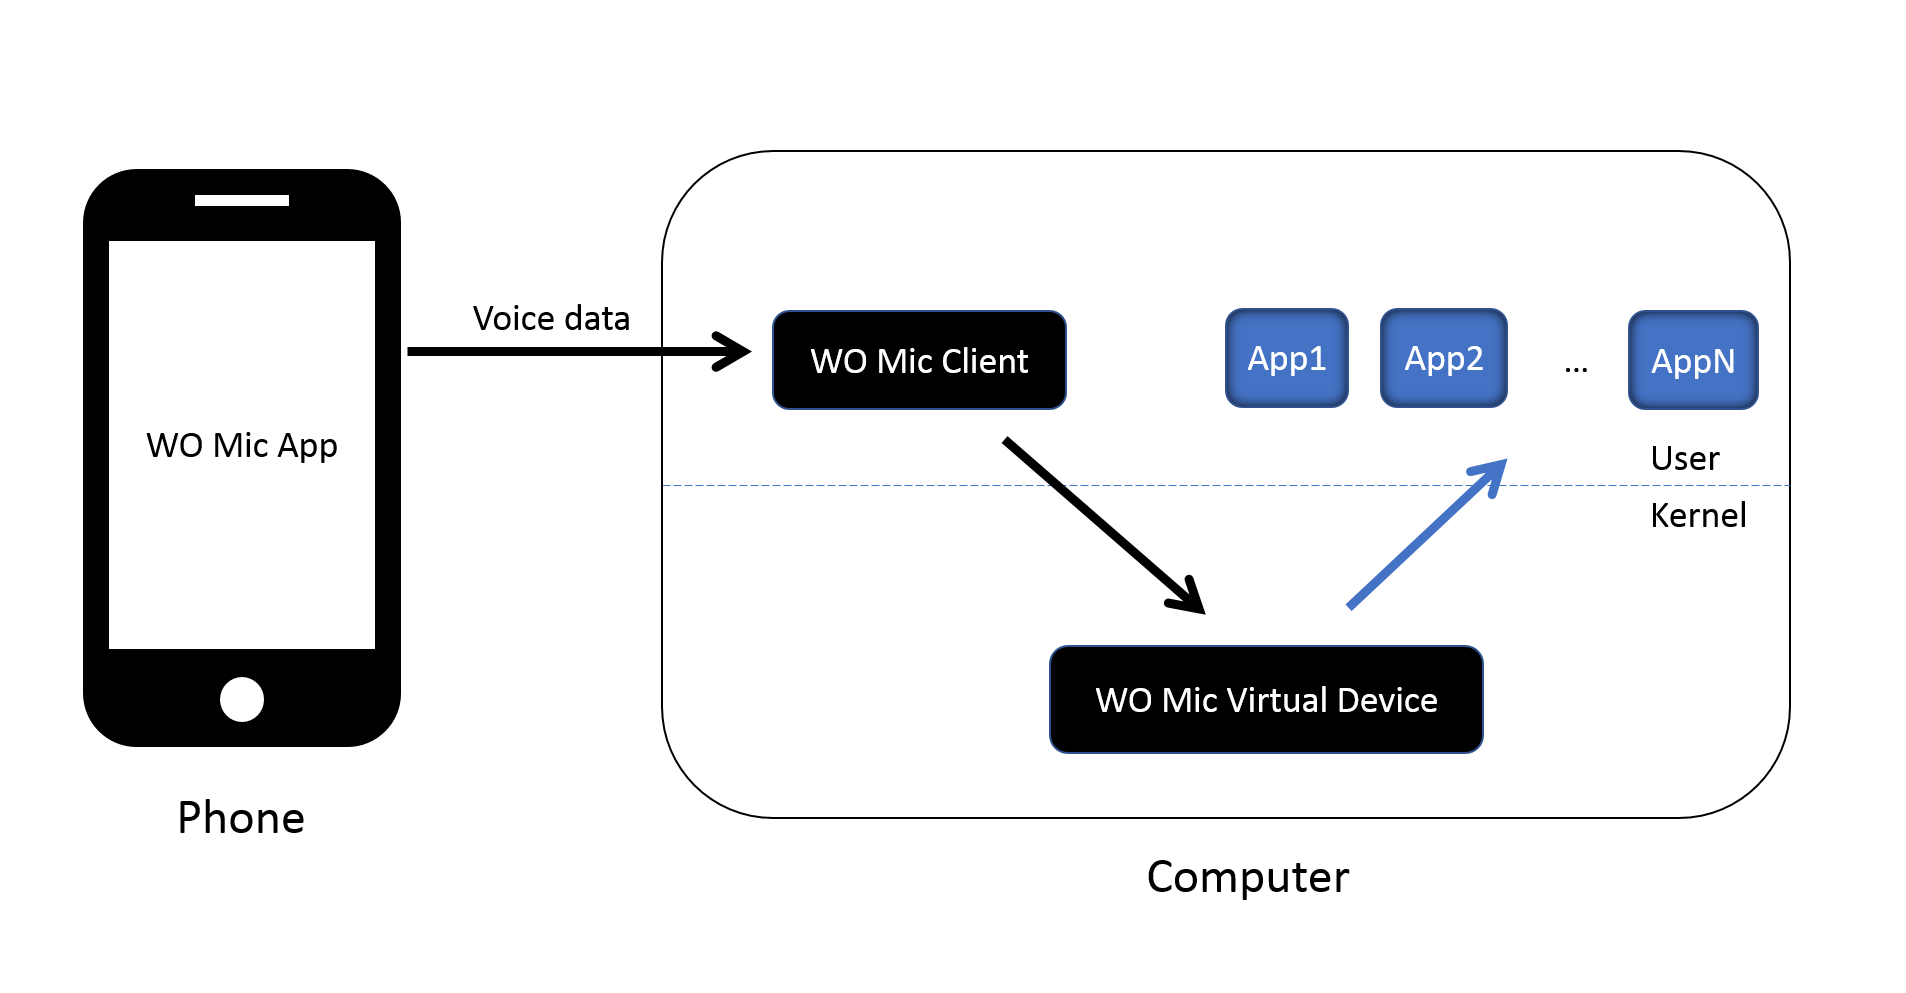
\includegraphics[width=0.65\textwidth]{Chapters/3CHP/Images/WOMICDiag.png}
        \caption{Flow of data in the components of the software\cite{WOMicFREE}}
        \label{fig:diagramWOMIC}
    \end{figure}
    In addition to this, is also necessary to install the drivers of the phone in used, if the connection is made over USB.
    \subsection*{}  

\subsection{Options}
\subsection{Amplifier circuits}
\subsection{Coupling} 

% \begin{figure}[!htb]
%     \centering 
%         \begin{subfigure}[c]{\textwidth}
%             \centering
%             \input{Sections/3Transforms/Images/DFTSymmetry.tex}
%             \caption{}
%             \label{subfig:dft}
%         \end{subfigure}
%         \begin{subfigure}[c]{0.45\textwidth}
%             \centering
%             \input{Sections/3Transforms/Images/DCT1Symmetry.tex}
%             \caption{}
%             \label{subfig:dct1}
%         \end{subfigure}
%         \begin{subfigure}[c]{0.45\textwidth}
%             \centering
%             \input{Sections/3Transforms/Images/DCT2Symmetry.tex}
%             \caption{}
%             \label{subfig:dct2}
%         \end{subfigure}
%         \begin{subfigure}[c]{0.45\textwidth}
%             \centering
%             \input{Sections/3Transforms/Images/DCT3Symmetry.tex}
%             \caption{}
%             \label{subfig:dct3}
%         \end{subfigure}
%         \begin{subfigure}[c]{0.45\textwidth}
%             \centering
%             \input{Sections/3Transforms/Images/DCT4Symmetry.tex}
%             \caption{}
%             \label{subfig:dct4}
%         \end{subfigure}
%         \caption{Sequences generated in the first step of Table \ref{tab:DFTDCT}for the DFT and different DCTs. Filled dots correspond to the original sequence ((a) - \emph{DFT}; (b)) - \emph{DCT-I}; (c)) - \emph{DCT-II}; (d)) - \emph{DCT-III}; (e)) - \emph{DCT-IV}).}
%     \label{fig:2NSeq}
% \end{figure}
% \begin{lstlisting}
%     ./aomenc <INPUT-FILE> -h <HEIGHT> -w <WIDTH> -o <OUTPUT-FILE> --limit=10 -p 1 --cpu-used=8 --i420 --q-hist=64 --end-usage=q --cq-level=<CQ-LEVEL>
% \end{lstlisting}
\clearpage
%\printbibliography[heading=subbibliography]
%\addcontentsline{toc}{section}{References}